\chapter{Conclusions and possible improvements}
\label{chap:ch6}


\textcolor{green}{aici trebuie sa spui pe scurt ce problema ai incercat sa rezolvi, ce metode ai folosit si abia  apoi ce rezultate ai obtinut (deci rezultatele sunt scrise, dar tb un text scurt despre problema si metoda; este o recomandarea in care Introducerea si Concluzia trebuie sa fie oarecum in oglinda, doar ca in introducere stilul de exprimare e intentional (vrei sa rezolvi, vrei sa dezvolti, asta e planul), iar in concluzie tonul e oarecum concluziv (am facut asta si am obtinut asta)}

In the end, GoogLeNet proved to not be a worthy architecture for the classification of cancer tumors in digital breast tomosynthesis images because of the low accuracy obtained. The highest accuracy obtained was 0.6321 and precision and recall for predicting cancer images were 0.6027 and 0.6087, respectively. I propose a different architecture, maybe DenseNet or ResNet to train and compare the results obtained by GoogLeNet. Additionally, I would increase the length of the dataset even more by including all the slices, keeping in mind the risk that some inputs might overpower others, especially considering the fact that the lowest number of slices an image has in the database is 22, and the highest number is 120.

As for EfficientDet, I am quite happy with the results of the trained model. I would maybe experiment with other types of EfficientDet, from D1 to D5. I do have some concerns, mainly the fact that the test loss seems to slightly increase from epoch to epoch while the train loss decreases. While the CosineAnnealing learning rate decay proved to work well with the model, I would experiment with other types of learning rate decay, such as OneCycle. The test loss obtained was 1.315 and the train loss was 0.2524. I would also experiment with different values for the anchor boxes.

\begin{figure}
    \centering
    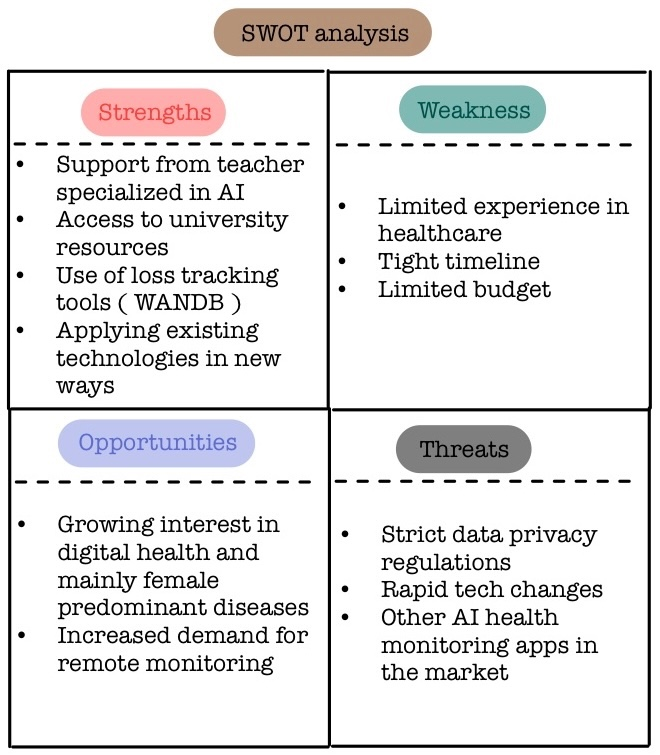
\includegraphics[width=0.5\linewidth]{figures/Figure54.png}
    \caption{SWOT analysis}
    \label{fig:fig44}
\end{figure}

\textcolor{green}{e ok swot-ul (figura si continutul ei), dar ar fi dragut sa adaugi si un paragraf textual care sa povesteasca continutul figurii si care sa zica ca toata povestea e rezumata in figura \ref{fig:fig44}}
